\section{Results}
\label{sec:auswertung}

\autoref{fig:camera_images} shows (cropped) images
from the \component{CCD camera}
of the laser beam hitting the \component{IR viewing card}.
In \autoref{fig:not_lasing} the laser is not lasing
and rather behaves like an LED.
After a threshold current,
the light intensity rises sharply,
as can be seen in \autoref{fig:lasing}.
The speckles indicate that the light is now monochromatic;
the laser is lasing.
%
The threshold current
    at this point in the procedure (before further calibration)
was determined to be \SI{35.2}{\milli\ampere}.

\begin{figure}
    \centering
    \begin{subfigure}{0.4\textwidth}
        \centering
        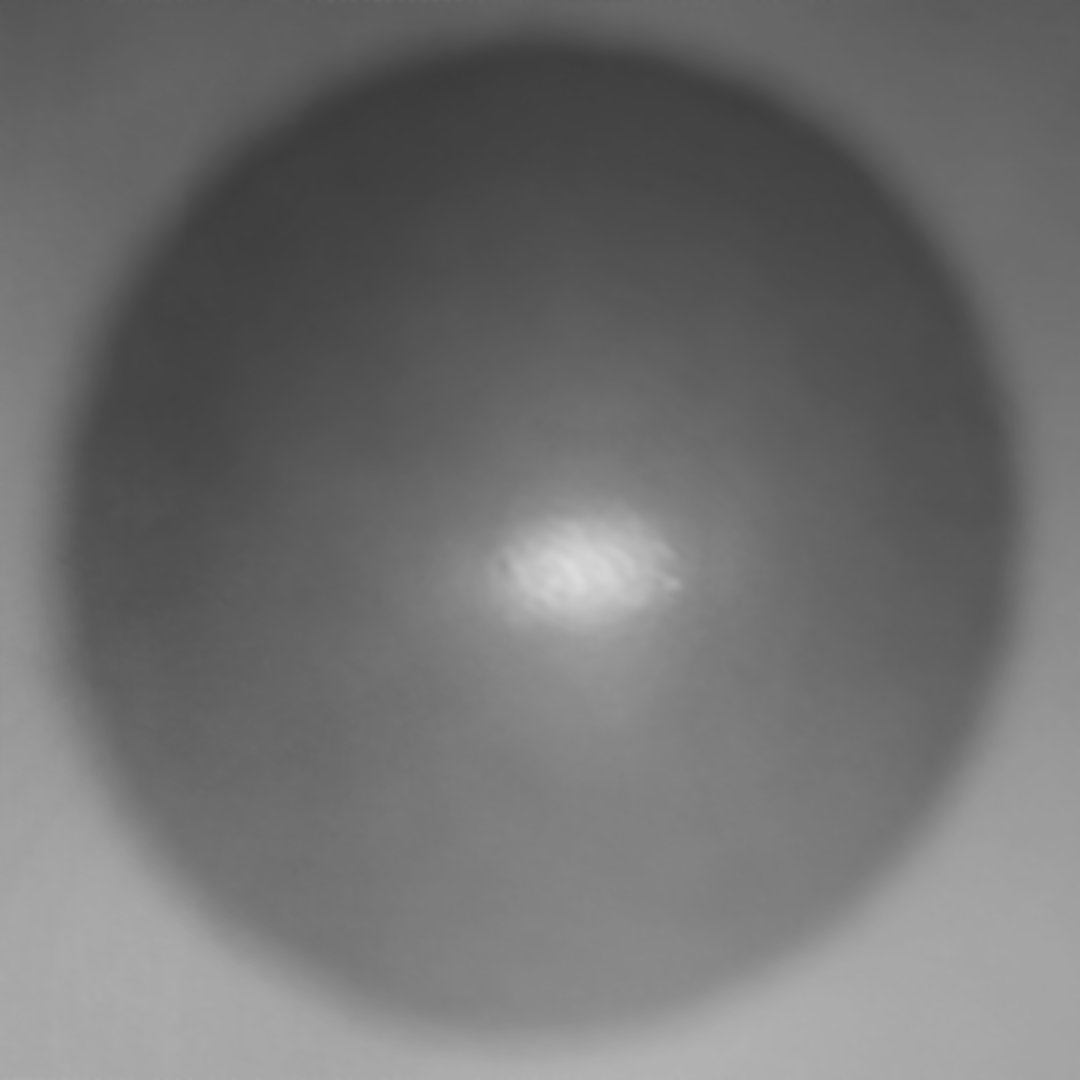
\includegraphics[width=0.65\textwidth]{content/img/not_lasing.jpg}
        \caption{Not lasing}
        \label{fig:not_lasing}
    \end{subfigure}
    \begin{subfigure}{0.4\textwidth}
        \centering
        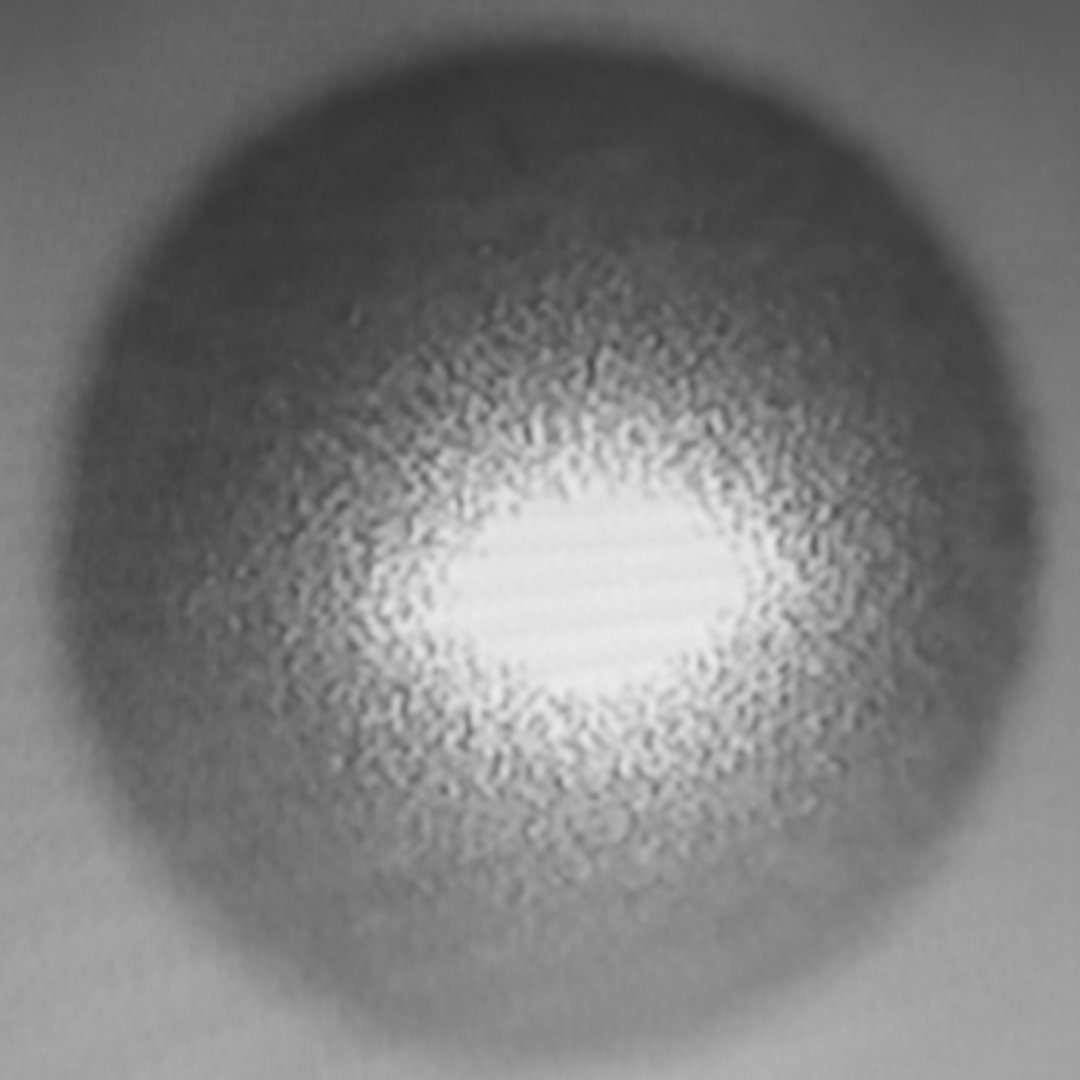
\includegraphics[width=0.65\textwidth]{content/img/lasing.jpg}
        \caption{Lasing}
        \label{fig:lasing}
    \end{subfigure}
    \caption{Camera images of the laser beam at different currents around the threshold value.}
    \label{fig:camera_images}
\end{figure}


% \subsection{Rubidium absorption spectrum}
At the end of the procedure,
the oscilloscope (see \autoref{fig:measurement}) shows the expected absorption lines (see \autoref{fig:measurement_lit});
all four peaks are positioned correctly and have appropriate relative heights.
In contrast to the reference,
a wider time range is displayed,
therefore revealing part of the mirrored absorption spectrum
as caused by the ramp function (yellow).

\begin{figure}
    \centering
    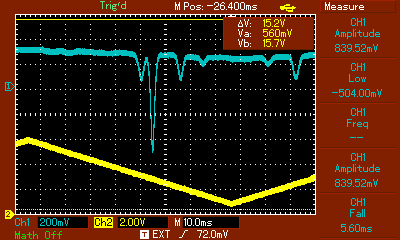
\includegraphics[width=0.75\textwidth, interpolate=false]{content/img/screenshot5.png}
    \caption{
        Oscilloscope screenshot depicting the measured spectrum in blue.
        The yellow line shows the \componentlabel{MONITOR OUTPUT} of the \component{Piezo Controller}.
    }
    \label{fig:measurement}
\end{figure}

\begin{figure}
    \centering
    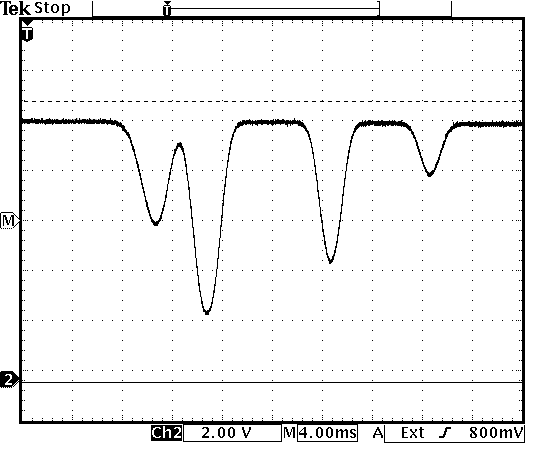
\includegraphics[width=0.75\textwidth]{content/img/p41_Fig14.png}
    \caption{Spectrum from the instructions for comparison \cite{versuchsanleitung}.}
    \label{fig:measurement_lit}
\end{figure}
